\begin{figure}[htbp]
\centering
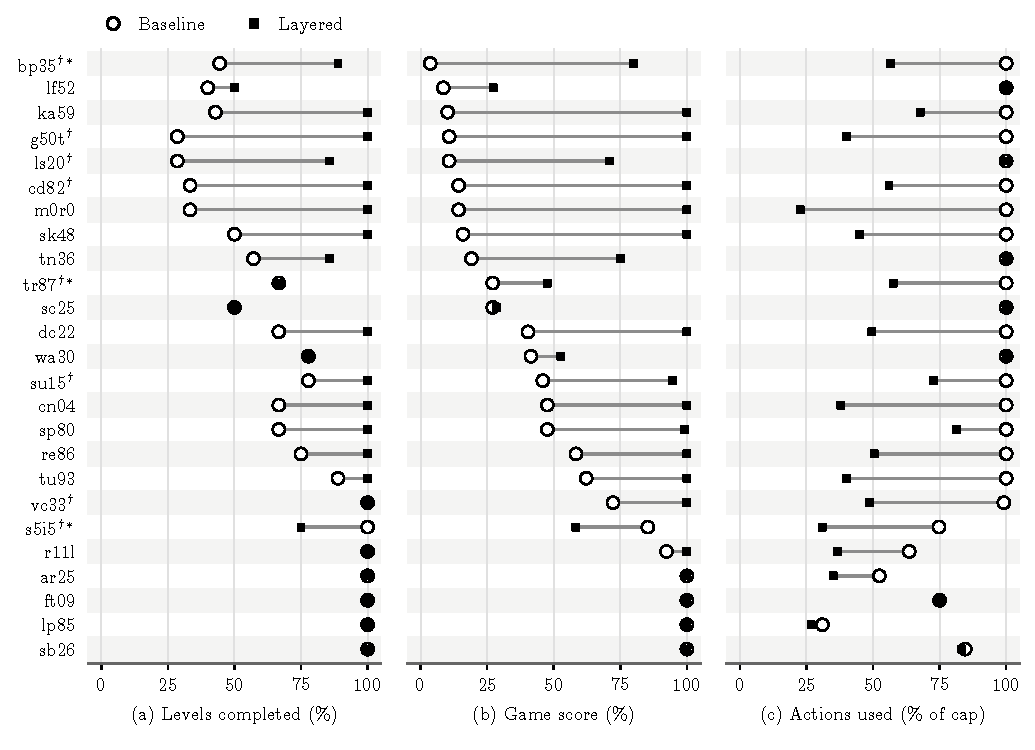
\includegraphics[width=\linewidth]{figures/per_game_outcomes.pdf}
\caption{\textbf{In most games the layered run completed more levels and scored higher while using fewer actions.} Each row compares one baseline run and one layered run on the same game. The rows run from the lowest baseline score to the highest. Open circles show the baseline results, filled squares show the layered results, and a line connects the two. The panels show (a) the percentage of levels completed, (b) the game score, and (c) the percentage of the game's action cap used. Both harnesses had the same cap for each game. A dagger marks games used or studied during development. An asterisk marks layered runs stopped by repeated timeouts; the figure reports their results at the point they stopped. The layered harness completed more levels in 15 games, the same number in nine, and fewer in one (\texttt{s5i5}). It scored higher in 20 games and used fewer actions in 19. The connecting lines show differences between two recorded runs; they do not show statistical uncertainty. Table~\ref{tab:layered-games} gives the exact values.}\label{fig:per-game-outcomes}
\end{figure}